\documentclass[letter,12pt]{article}
%
\usepackage[left=1in, top=1in, bottom=1in, right=1in]{geometry}

% packages 
\usepackage{latexsym,amssymb,amsmath,color}
%\usepackage{theorem}
\usepackage{graphicx}
%\usepackage[colorlinks=true]{hyperref}
%\hypersetup{urlcolor=blue, citecolor=red}
%\usepackage{algorithmic}
%\usepackage{algorithm}
\usepackage{cite}
\usepackage{verbatim}
\usepackage[table]{xcolor}

% -------------- macros
\newcommand{\p}{\partial}
\def\Cb{\overline{C}}

\newcommand{\R}{\mathbb{R}}
\newcommand{\N}{\mathbb{N}}
\newcommand{\cov}{\mathrm{cov}}
\newcommand{\iid}{\stackrel{iid}{\sim}}
\newcommand{\F}{\mathcal{F}}%
\newcommand{\be}{\begin{equation}}
\newcommand{\ee}{\end{equation}}
\newcommand{\bea}{\begin{eqnarray}}
\newcommand{\eea}{\end{eqnarray}}
%\newcommand{\p}{\partial}
\newcommand{\ttt}{\tilde}
\newcommand{\rev}[1]{{\color{blue}{#1}}}
%
\def\Wb{\overline{W}}
\def\td{\tilde \delta}
\def\tL{\tilde L}
\def\tU{\tilde U}
\def\tt{\tilde t}
\def\Vector#1{\mbox{\boldmath $#1$}}
\def\vH{{\Vector H}}
\def\vx{{\Vector x}}
\def\vy{{\Vector y}}
\def\vz{{\Vector z}}
\def\vj{{\Vector j}}
\def\vk{{\Vector k}}
\def\vt{{\Vector t}}
\def\ve{{\Vector e}}
\def\vb{{\Vector b}}
\def\vg{{\Vector g}}
\def\vn{{\Vector n}}
\def\vp{{\Vector p}}
\def\vr{{\Vector r}}
\def\vS{{\Vector S}}
\def\vV{{\Vector V}}
\def\vY{{\Vector Y}}
\def\vX{{\Vector X}}
\def\vv{{\Vector v}}
\def\vu{{\Vector u}}
\def\vQ{{\Vector Q}}
\def\vZ{{\Vector Z}}
\def\vN{{\Vector N}}
\def\vF{{\Vector F}}
\def\vC{{\Vector C}}
\def\vq{{\Vector q}}
\def\vom{{\Vector \omega}}
\def\vtau{{\Vector \tau}}
\def\F{{\rm\bf F}}
\def\sech{{\rm sech}}
\def\funnyzeta{\varsigma}
\def\tQ{\stackrel{\ldots}{Q}}
%
\def\Re{{\rm Re}}
\def\Sc{{\rm Sc}}
\def\Pe{{\rm Pe}}
\def\Pr{{\rm Pr}}
\def\Da{{\rm Da}}
\def\rf{{\rm ref}}
\def\eps{{\varepsilon}}
\def\ep{\epsilon'}
\def\O{{\rm O}}
\def\1{{\rm 1}}
\def\so{^{\rm (0)}}
\def\s1{^{\rm (1)}}
\def\d{{\rm d}}
\def\ttm{^{{\rm ttm}}}
\def\img{^{\rm im}}
\def\si{^{\rm si}}
%
\def\ol{\overline}
%
\def\tn{^{n}}
\def\tnm{^{n-1}}
\def\new#1{{\bf #1}}
%\def\new#1{{#1}}

\renewcommand{\L}{\mathcal{L}}
\newcommand{\Q}{\mathcal{Q}}
\newcommand{\U}{\mathcal{U}}
\newcommand{\G}{\mathcal{N}}
\newcommand{\V}{\mathcal{V}}
\renewcommand{\P}{\mathrm{P}}
\newcommand{\B}{\mathcal{B}}
\renewcommand{\vec}[1]{{\mathchoice
                     {\mbox{\boldmath$\displaystyle{#1}$}}
                     {\mbox{\boldmath$\textstyle{#1}$}}
                     {\mbox{\boldmath$\scriptstyle{#1}$}}
                     {\mbox{\boldmath$\scriptscriptstyle{#1}$}}}}
\newcommand{\var}[1]{{\mathrm{Var}}\left( {#1} \right)}
\newcommand{\normim}[1]{\left\| {#1} \right\|_{\scriptscriptstyle L^{2}(\Omega^{*})}}
\newcommand{\avemu}[1]{\mathrm{E}\left({#1}\right)}
\newcommand{\ave}[1]{\left\langle {#1} \right\rangle}
\newcommand{\prob}[1]{\mathrm{Prob}\left\{ {#1} \right\}}
\newcommand{\ind}[1]{\mathrm{\chi}_{\scriptscriptstyle {#1} }}
\newcommand{\NISP}{\mathcal{S}}
\newcommand{\xxi}{\vec{\xi}}
\newcommand{\ip}[2]{\left( {#1}, {#2} \right)}
\newcommand{\ipmu}[2]{\left( {#1}, {#2} \right)_\mu}
\newcommand{\norm}[1]{\left\| {#1} \right\|_{\scriptscriptstyle L^{2}(\Omega)}}
\newcommand{\normone}[1]{\left\| {#1} \right\|_{\scriptscriptstyle 1}}
\newcommand{\pard}[2]{\frac{\partial{#1}}{\partial{#2}}}
%
%\newcommand{\be}{\begin{equation}}
%\newcommand{\ee}{\end{equation}}
%\newcommand{\bea}{\begin{eqnarray}}
%\newcommand{\eea}{\end{eqnarray}}
%\newcommand{\p}{\partial}
%\newcommand{\ttt}{\tilde}
%
\def\Wb{\overline{W}}
\def\td{\tilde \delta}
\def\tL{\tilde L}
\def\tU{\tilde U}
\def\tt{\tilde t}
\def\Vector#1{\mbox{\boldmath $#1$}}
\def\vH{{\Vector H}}
\def\vx{{\Vector x}}
\def\vy{{\Vector y}}
\def\vz{{\Vector z}}
\def\vj{{\Vector j}}
\def\vk{{\Vector k}}
\def\vt{{\Vector t}}
\def\ve{{\Vector e}}
\def\vb{{\Vector b}}
\def\vg{{\Vector g}}
\def\vn{{\Vector n}}
\def\vp{{\Vector p}}
\def\vr{{\Vector r}}
\def\vS{{\Vector S}}
\def\vV{{\Vector V}}
\def\vY{{\Vector Y}}
\def\vX{{\Vector X}}
\def\vv{{\Vector v}}
\def\vu{{\Vector u}}
\def\vQ{{\Vector Q}}
\def\vZ{{\Vector Z}}
\def\vN{{\Vector N}}
\def\vF{{\Vector F}}
\def\vC{{\Vector C}}
\def\vq{{\Vector q}}
\def\vom{{\Vector \omega}}
\def\vtau{{\Vector \tau}}
\def\F{{\rm\bf F}}
\def\sech{{\rm sech}}
\def\funnyzeta{\varsigma}
\def\tQ{\stackrel{\ldots}{Q}}
%
\def\Re{{\rm Re}}
\def\Sc{{\rm Sc}}
\def\Pe{{\rm Pe}}
\def\Pr{{\rm Pr}}
\def\Da{{\rm Da}}
\def\rf{{\rm ref}}
\def\eps{{\varepsilon}}
\def\ep{\epsilon'}
\def\O{{\rm O}}
\def\1{{\rm 1}}
\def\so{^{\rm (0)}}
\def\s1{^{\rm (1)}}
\def\d{{\rm d}}
\def\ttm{^{{\rm ttm}}}
\def\img{^{\rm im}}
\def\si{^{\rm si}}
%
\def\ol{\overline}
%
\def\tn{^{n}}
\def\tnm{^{n-1}}
\def\new#1{{\bf #1}}
\newcommand{\todo}[1]{\scshape\color{red}{#1}}
%
 \def\ol{\overline}
 \def\no{\noindent}
 \def\qd{\dot{Q}}
% ----------------- end macros

\usepackage[table]{xcolor}
\usepackage{relsize}
\usepackage{bm}
\usepackage{mathrsfs}

 \def\ol{\overline}
 \def\no{\noindent}
 \def\qd{\dot{Q}}
%%%%%%%FLOW DIAGRAM%%%%%%%%%%
\usepackage[latin1]{inputenc}
\usepackage{tikz}
%\usepackage[table]{xcolor}
\usetikzlibrary{shapes,arrows}
% Define block styles
\tikzstyle{decision} = [diamond, draw, fill=blue!20, 
   text width=5.0em, text badly centered, node distance=3cm, inner sep=0pt]
\tikzstyle{block} = [rectangle, draw, fill=cyan!20, 
   text width=9.0em, text centered, rounded corners]
\tikzstyle{line} = [draw, -latex']
\tikzstyle{cloud} = [draw, ellipse,fill=red!20, node distance=3cm,
   minimum height=2em]
%%%%%%%%%%%%%%%%%%%%%%%%%%

%-------------------------------------------------------------------
\begin{document}

\thispagestyle{empty}
\begin{center}
\textsc{
Uncertainty Analysis in Non-Equilibrium Molecular Dynamics Simulations for
Thermal Transport
}

\bigskip 
\bigskip 

Manav Vohra$^{1}$, Ali Y. Nobakht$^{2}$, Seungha Shin$^{2}$, Sankaran Mahadevan$^{1}$

\bigskip
\bigskip

\normalsize
$^1$Department of Civil and Environmental Engineering\\
Vanderbilt University\\
Nashville, TN 37235\\

\bigskip

$^2$Department of Mechanical, Aerospace, and Biomedical Engineering\\
The University of Tennessee\\
Knoxville, TN 37996\\

\bigskip

\end{center}

\vspace{6cm}

\begin{tabbing}
Corresponding Author: \hspace{5mm} \= Sankaran Mahadevan\\
       \>  Department of Civil and Environmental Engineering\\
       \>  Vanderbilt University\\
       \>  272 Jacobs Hall, VU Mailbox: PMB 351831 \\
       \>  Nashville, TN 37235 \\
       \> \\
Phone: \> (615) 322-3040 \\
Fax:   \> (615) 343-3773 \\
Email: \>  sankaran.mahadevan@vanderbilt.edu   \\
\\
Submitted to: \> \textit{International Journal of Heat and Mass Transfer} \\
\>  April 2018\\

\bigskip
\end{tabbing}

\clearpage



\baselineskip=22pt

\tableofcontents

\section*{Abstract}

Bulk thermal conductivity estimates based on predictions from non-equilibrium molecular dynamics (NEMD)
using the so-called direct method are known to be severely under-predicted since finite simulation
length-scales are unable to mimic bulk transport. Moreover, subjecting the system to a temperature gradient
by means of thermostatting tends to impact phonon transport adversely.  Additionally, NEMD predictions
are tightly coupled with the choice of the inter-atomic potential and the underlying values associated with its
parameters. In the case of silicon (Si), nominal estimates of the Stillinger-Weber (SW) potential parameters are largely based 
on a constrained regression approach aimed at agreement with experimental data while ensuring structural
stability. However, this approach has its shortcomings and it may not be ideal to use the same set of parameters
 to study a wide variety of Si-based
systems subjected to different thermodynamic conditions. 
In this study, NEMD simulations are performed on a Si bar to investigate the impact of bar-length,
and the applied thermal gradient on the discrepancy between predictions and the available measurement 
for bulk thermal conductivity at 300~K by constructing statistical response surfaces at different temperatures. 
The approach helps quantify the discrepancy, observed to be largely dependent on the system-size, with minimal
computational effort. A computationally efficient approach based on derivative-based sensitivity measures to
construct a reduced-order polynomial chaos surrogate for NEMD predictions is also presented. The surrogate
is used to perform parametric sensitivity analysis, forward propagation of the uncertainty, and calibration of the important SW potential parameters in a 
Bayesian setting. It is found that only two (out of seven) parameters contribute significantly to the uncertainty
in bulk thermal conductivity estimates for Si. 
\clearpage

\section{Introduction}
\label{sec:intro}

\begin{comment}
1. Background on use of MD simulations for thermal transport, preferred for studying
thermal transport by phononic interactions (refer notes from book suggested by Amuthan)


2. One approach to NEMD is the Direct Method, commonly used for estimating the bulk
thermal conductivity. A brief discussion on the direct method and associated pros and cons
(notes from Dellan's paper and book suggested by Amuthan) 
Predictions impacted by the choice of potential, values of
individual parameters, size, and potentially due to duration and applied thermal gradients
(cite Amuthan book, Francesco's paper, McGaughey's paper). 
Errors are introduced by thermostatting (Amuthan book). Nominal value of SW potential parameters based on fitting against experiments and to ensure structural stability etc. (SW paper)

3. Motivate uncertainty analysis and briefly discuss and cite recent efforts (Francesco, Kirby,
Murthy). Highlight focus and key contributions of the present work and how it differs from
those efforts. 

4. Section-wise overview of the paper.  
\end{comment}

Classical Molecular Dynamics (MD) is commonly used to study thermal transport by means of phonons in material 
systems comprising non-metallic elements such as carbon, silicon, germanium.  
\bigskip
\bigskip
%
%
%\input{bg}
%\bigskip
%\bigskip
%
%
%\input{method}
%\bigskip
%\bigskip
%
%
%\input{examples}
%\bigskip
%\bigskip
%
%
%\input{app}
%\bigskip
%\bigskip
%
%
%\section{Summary and Discussion}
\label{sec:disc}

In this paper, we have attempted to identify and address some of the challenges
pertaining to uncertainty quantification of bulk thermal conductivity predictions 
using non-equilibrium molecular dynamics (NEMD) simulations. Specifically, we focused
on investigating the impact of system size, and fluctuations in the applied temperature
gradient on predictions. In order to quantify the discrepancy between NEMD
predictions and experiments, response surfaces were  
constructed at bulk temperatures, $T$ = 300~K, 500~K, and 1000~K.  
It was found that the discrepancy is predominantly impacted by size while the 
effect of fluctuations in the applied temperature gradient is negligible in the considered
interval. The response surface approach presented here relies on a small number of
MD runs and enables an accurate estimation of discrepancy at a given temperature
and a point in the 2D parameter space described by system-size and the applied
temperature gradient. 

A possible enhancement of nominal SW parameter estimates for a given application
and the choice of material system is also highlighted in this work. To enable this,
we focus our efforts on understanding the sensitivity of predictions on individual potential
parameters. In order to reduce the computational effort, we estimate the DGSMs
 and hence the upper bound
on Sobol\textquotesingle~total-effect sensitivity index using random samples in the 7D parameter space. 
While individual measures for the 7 parameters are not too distant from each other, the predictions
seem to be most sensitive towards $\gamma$. Sensitivity measures for $\alpha$,
$\lambda$, $q$, and $A$ are found to be comparable while those for $B$ and $p$
are relatively small. 

A polynomial chaos surrogate model for the bulk thermal conductivity (observable)
as a function of SW potential
parameters at the bulk temperature of 300~K is constructed. The surrogate helps reduce the
computational effort required for forward propagation of the uncertainty from
parameters to the observable as well as for estimating the Sobol\textquotesingle~sensitivity indices.
Furthermore, the surrogate could be used to accelerate parameter calibration in a
Bayesian setting. However, since the surrogate relies on NEMD predictions, the
underlying computational effort is nevertheless significantly large. To circumvent
this challenge, we exploit our initial findings based on DGSM and construct
a reduced-order surrogate in 5 dimensions by fixing the parameters, $B$ and $p$.
We verify its accuracy by estimating the relative
L-2 norm of the error between NEMD predictions in the full space and the reduced-order
surrogate predictions, and by comparing the probability density of the
bulk thermal conductivity in Figure~\ref{fig:verify}. Furthermore, our initial
sensitivity trends based on DGSM-analysis using 25 samples seem to agree favorably
with Sobol\textquotesingle~sensitivity analysis based on 10$^{6}$ samples. Hence, it can be said
that DGSM-based analysis with a few samples could offer huge computational gains
by reliably reducing the dimensionality of a surrogate for uncertainty analysis. 

Finally, we highlight key aspects of parameter calibration in a Bayesian setting.
The underlying motivation stems from the fact that the nominal estimates of the SW
parameters did not consider measurement error, simulation noise, model form error,
and parametric uncertainties. Calibration in a Bayesian framework allows us to
incorporate such errors and uncertainties in an efficient manner and provides
a joint posterior distribution of the uncertain parameters. To minimize computational
costs pertaining to the calibration process, we suggest the following sequence of
steps: First, perform DGSM analysis to 
identify parameters that are not so important. Second, construct a reduced-order
surrogate based on DGSM-analysis and verify its accuracy. Third, compute the
Sobol\textquotesingle~sensitivity indices using the surrogate to identify parameters for calibration. 
Fourth, construct a second surrogate in the reduced subspace described by the
calibration parameters, and quantify the surrogate error to be accounted for
in calibration. Fifth, evaluate the joint posterior using an efficient MCMC-based algorithm
such as adaptive Metropolis~\cite{Haario:2001} and its variants~\cite{Haario:2006, Green:2001}.

It is important to note that the strategies presented 
in this work are not restricted to a Si bar and the Stillinger-Weber potential, and
could be extended to a wide range of applications and inter-atomic potentials for
the purpose of uncertainty quantification. 


%\bigskip
%\bigskip
%
%\section*{Acknowledgment}
\label{sec:ack}

M. Vohra and S. Mahadevan gratefully acknowledge funding support from the
National Science Foundation Award $\#$. Molecular
dynamics simulations were performed using resources at the advanced computing
center for research and education (ACCRE) at Vanderbilt University. 
M. Vohra is grateful to the ACCRE staff for their technical guidance
and support. He would also like to sincerely thank Dr. Alen Alexanderian for
insightful discussions pertaining to the derivative-based sensitivity analysis
aspect of this work.  



%\bigskip
%\bigskip
%
%\bibliographystyle{unsrt}
%\bibliography{REFER}
%
%\clearpage
%
%%%%%%%%%%%%%%%%%%%%%%%%%%%%%%%%%%%%%%%%%%%%%%%%%%%%%%%%%%%%%%%%%%%%%%%%%%
 
\begin{figure}[p]
\begin{center}
\begin{tabular}{cc}
  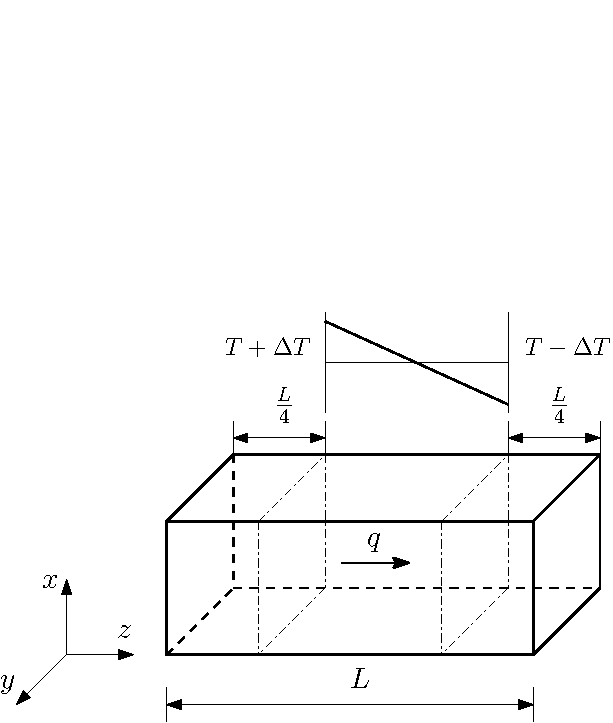
\includegraphics[width=0.48\textwidth]{./Figures/schematic}
  &
  \hspace{3mm}
  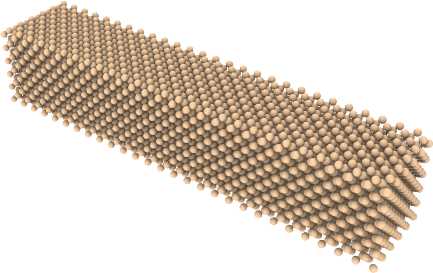
\includegraphics[width=0.40\textwidth]{./Figures/Sibar_05}
  \\ (a) & (b)
  \end{tabular}
\caption{(a) Schematic illustration of the set-up for evaluating thermal conductivity of Si using NEMD. (b) 
Arrangement of Si atoms prior to the application of thermal gradient.}
\label{fig:setup}
\end{center}
\end{figure}

\clearpage

%%%%%%%%%%%%%%%%%%%%%%%%%%%%%%%%%%%%%%%%%%%%%%%%%%%%%%%%%%%%%%%%%%%%%%%%%

\begin{figure}[p]
 \begin{center}
  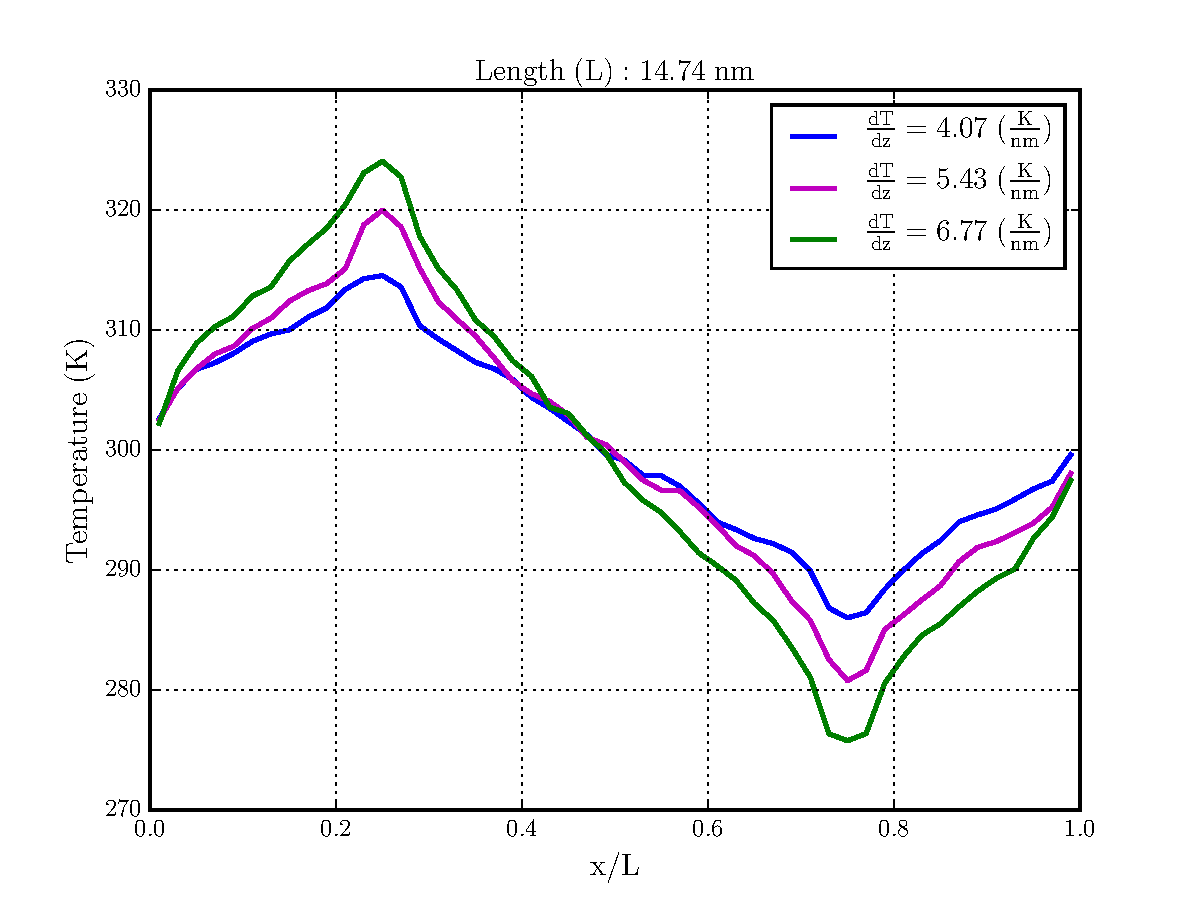
\includegraphics[width=0.70\textwidth]{./Figures/temp_plot}
\caption{Temperature distribution along a Si bar of length 14.74~nm for different scenarios of applied 
thermal gradient.}
\label{fig:kapitza}
\end{center}
\end{figure}


\clearpage

%%%%%%%%%%%%%%%%%%%%%%%%%%%%%%%%%%%%%%%%%%%%%%%%%%%%%%%%%%%%%%%%%%%%%%%%%

\begin{figure}[p]
\begin{center}
\begin{tabular}{cc}
  \hspace{-12mm}
  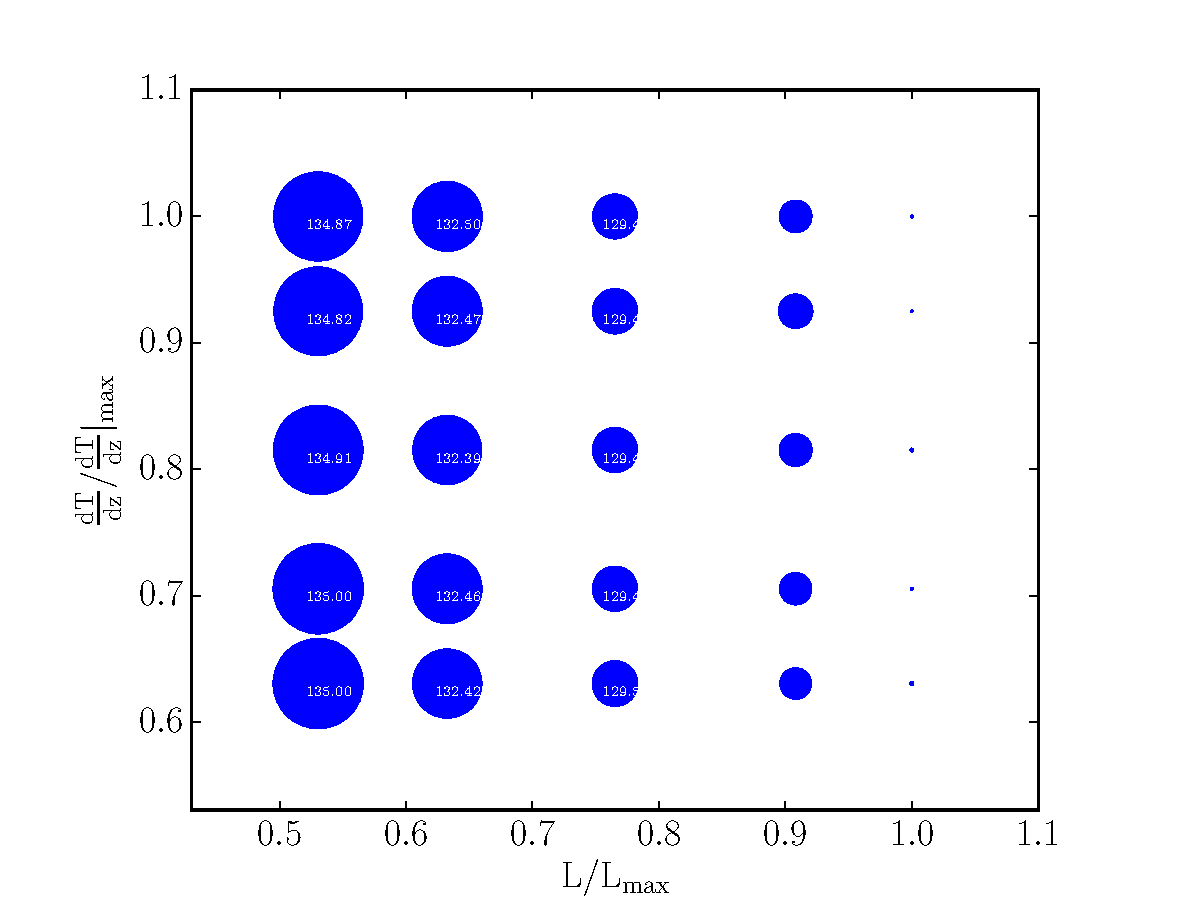
\includegraphics[width=0.60\textwidth]{./Figures/realz_quad300K}
  &
  \hspace{-9mm}
  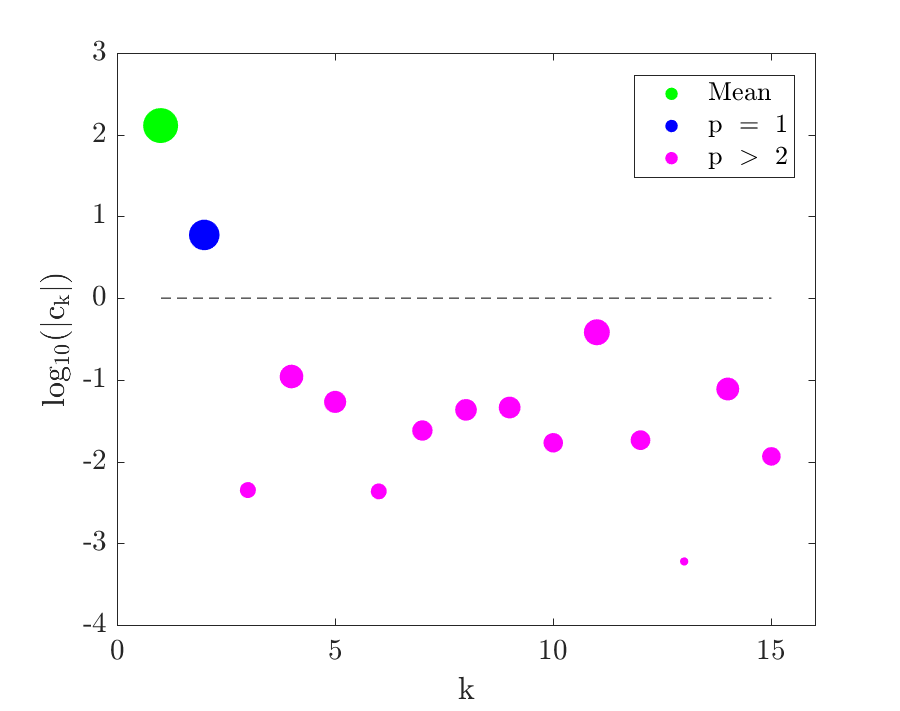
\includegraphics[width=0.56\textwidth]{./Figures/PCspectrum_300}
  \\ (a) & (b)
  \end{tabular}
\caption{(a) Realizations of discrepancy in bulk thermal conductivity at the Gauss-Legendre quadrature notes are
depicted using circles. The size of the circle in each case is proportional to the discrepancy estimate, also provided
 in cases where it is observed to be relatively large. (b) Spectrum of PC coefficients is depicted using circles of
 varying sizes, proportional to the log value of their magnitude. The computations were performed at 300 K.}
\label{fig:rs1}
\end{center}
\end{figure}

\clearpage

%%%%%%%%%%%%%%%%%%%%%%%%%%%%%%%%%%%%%%%%%%%%%%%%%%%%%%%%%%%%%%%%%%%%%%%%%

\begin{figure}[p]
\begin{center}
\begin{tabular}{cc}
 \hspace{-10mm}
  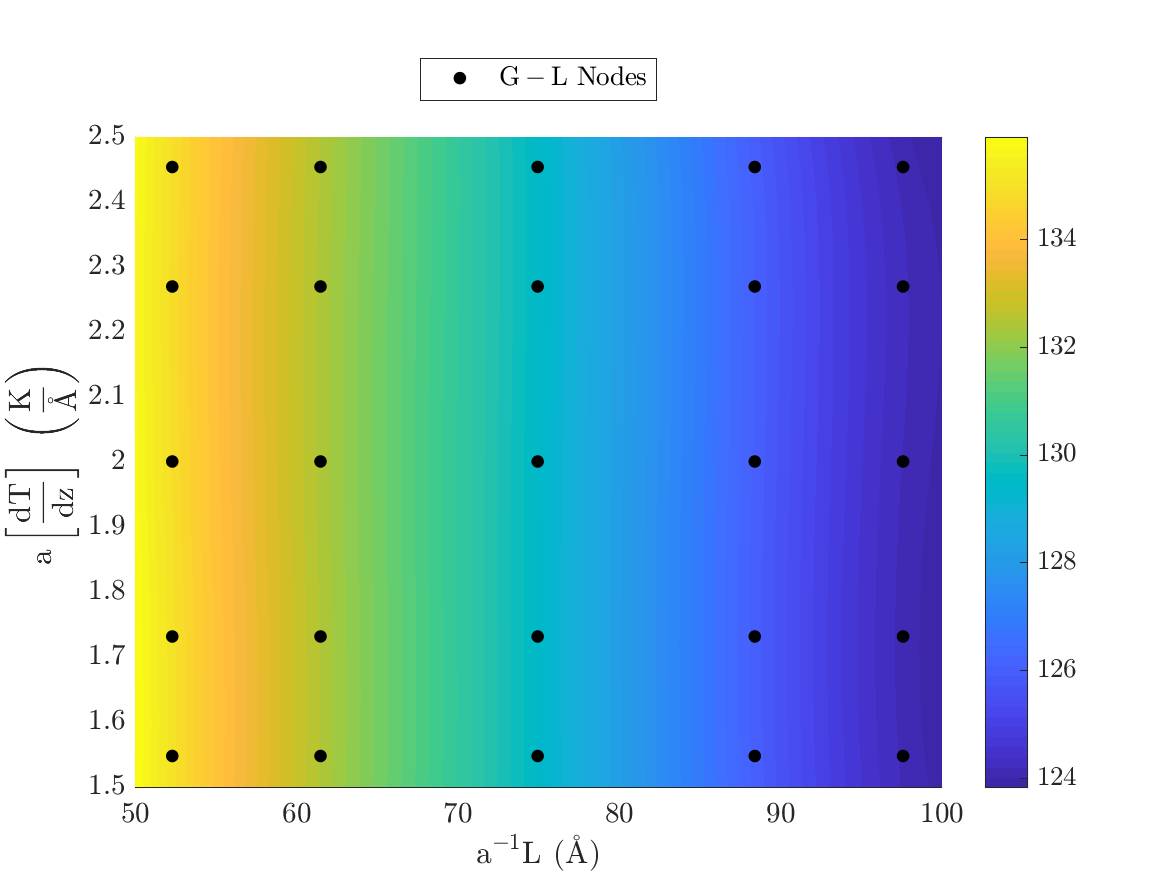
\includegraphics[width=0.55\textwidth]{./Figures/err2D_300}
  &
  %\hspace{-9mm}
  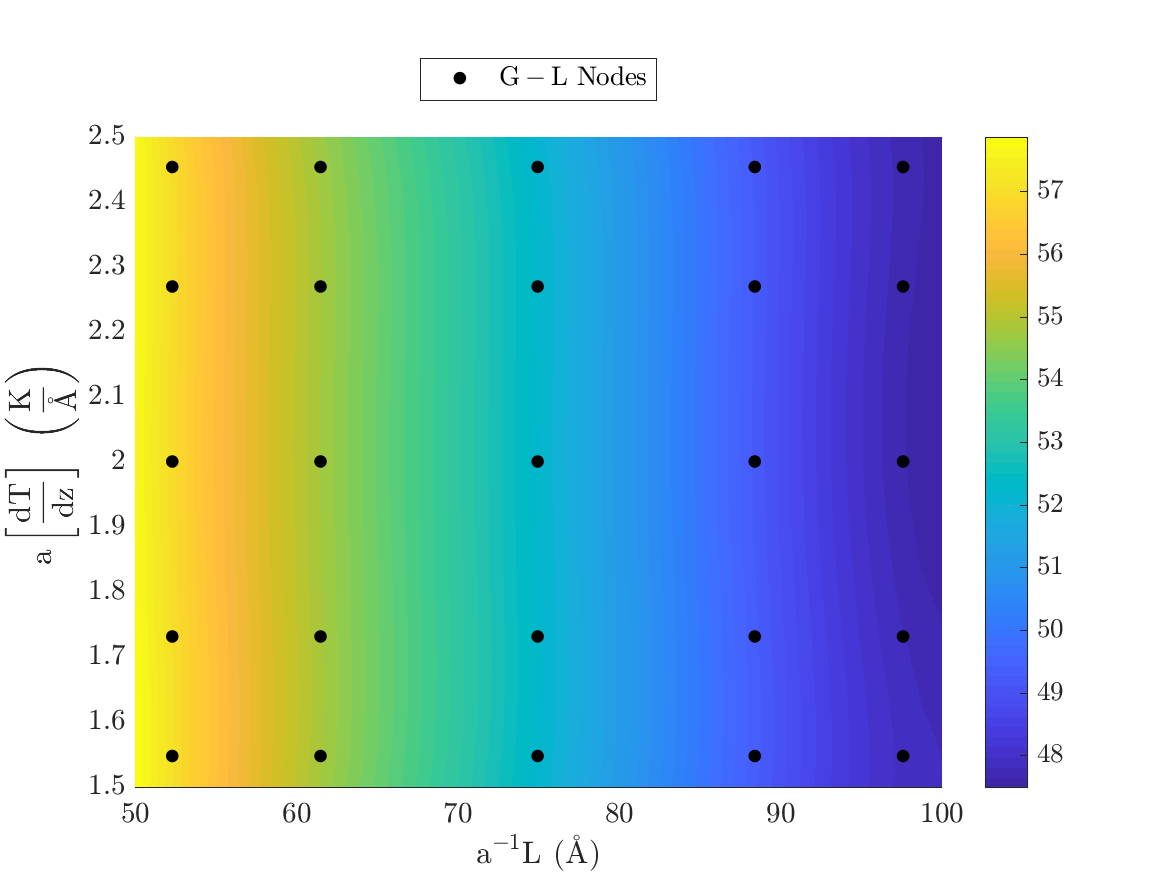
\includegraphics[width=0.55\textwidth]{./Figures/err2D_500}
  \\ (a) & (b)
  \end{tabular}
  \\ \vspace{1mm}
  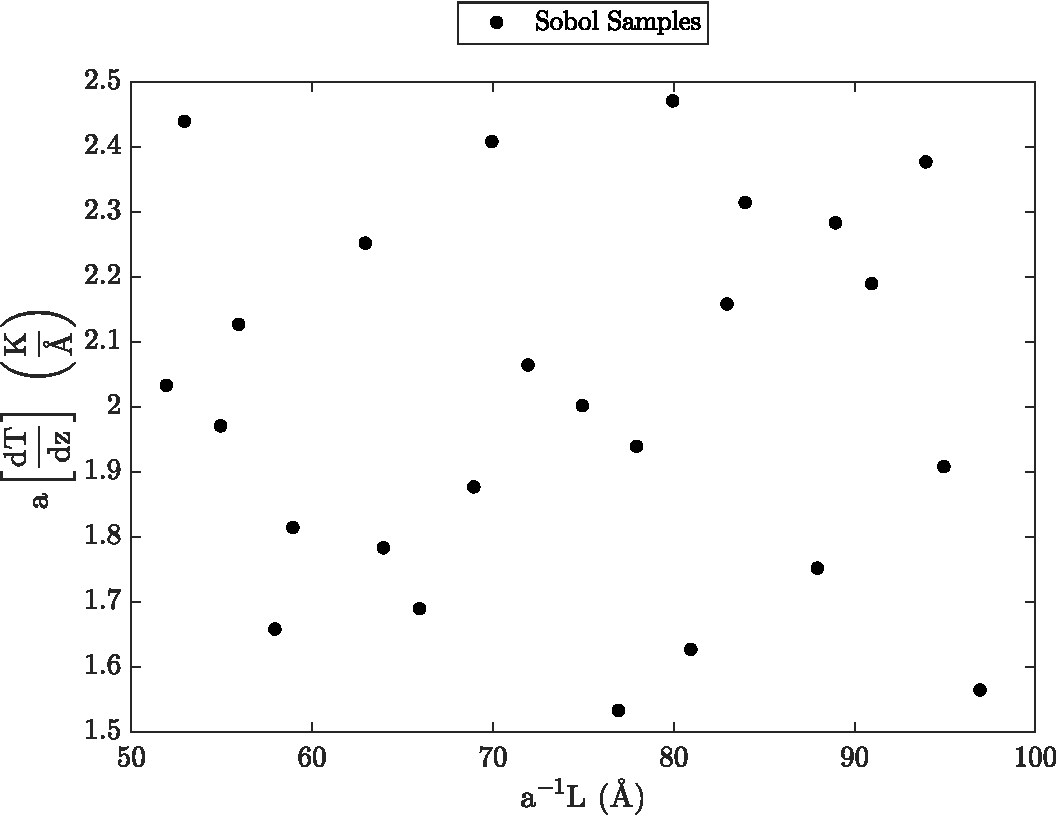
\includegraphics[width=0.50\textwidth]{./Figures/err2D_s}
  \\ (c)
\caption{Response surface of the discrepancy in bulk thermal conductivity at (a) $T$ = 300~K and
 (b) $T$ = 500~K. Gauss-Legendre quadrature nodes are highlighted in both cases. (c) Sobol samples
 in the 2D domain used for verifying the accuracy of the response surfaces.}
\label{fig:rs2}
\end{center}
\end{figure}

\clearpage

%%%%%%%%%%%%%%%%%%%%%%%%%%%%%%%%%%%%%%%%%%%%%%%%%%%%%%%%%%%%%%%%%%%%%%%%%

\begin{figure}[p]
\begin{center}
\begin{tabular}{cc}
 \hspace{-10mm}
  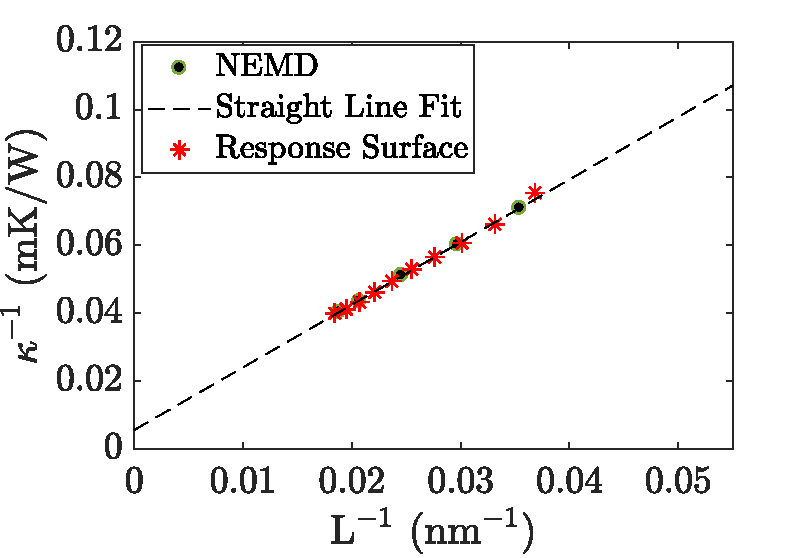
\includegraphics[width=0.50\textwidth]{./Figures/kinv_300}
  &
  %\hspace{-9mm}
  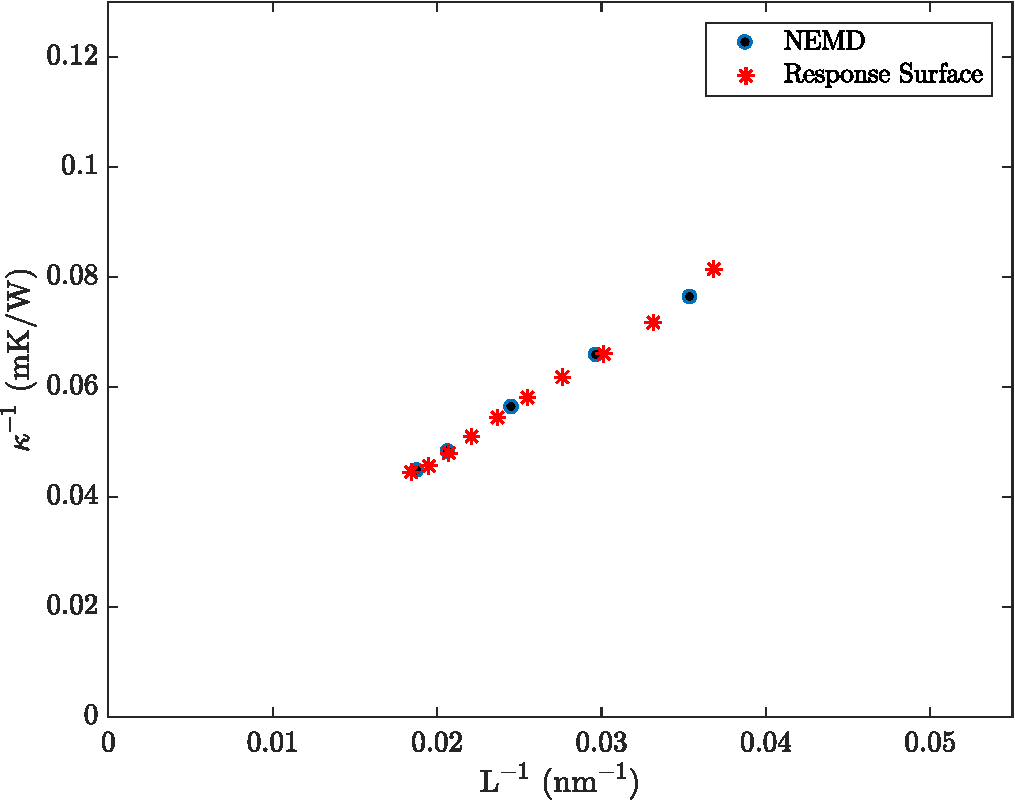
\includegraphics[width=0.50\textwidth]{./Figures/kinv_500}
  \\ (a) & (b)
  \end{tabular}
 \caption{Inverse of the bulk thermal conductivity estimates are plotted against the inverse of Si bar length
 using predictions from NEMD as well as estimates from the response surface at (a)  $T$ = 300~K and 
 (b) $T$ = 500~K.}
\label{fig:rs3}
\end{center}
\end{figure}

\clearpage

%%%%%%%%%%%%%%%%%%%%%%%%%%%%%%%%%%%%%%%%%%%%%%%%%%%%%%%%%%%%%%%%%%%%%%%%%
 
\begin{figure}[p]
\begin{center}
\begin{tabular}{cc}
  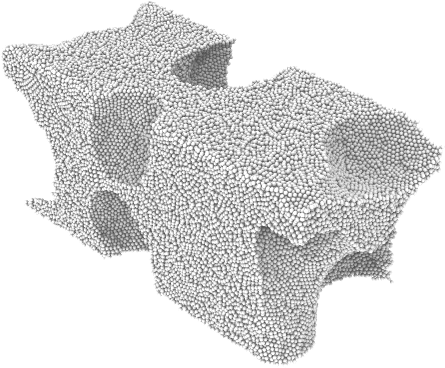
\includegraphics[width=0.40\textwidth]{./Figures/unstable}
  &
  \hspace{3mm}
  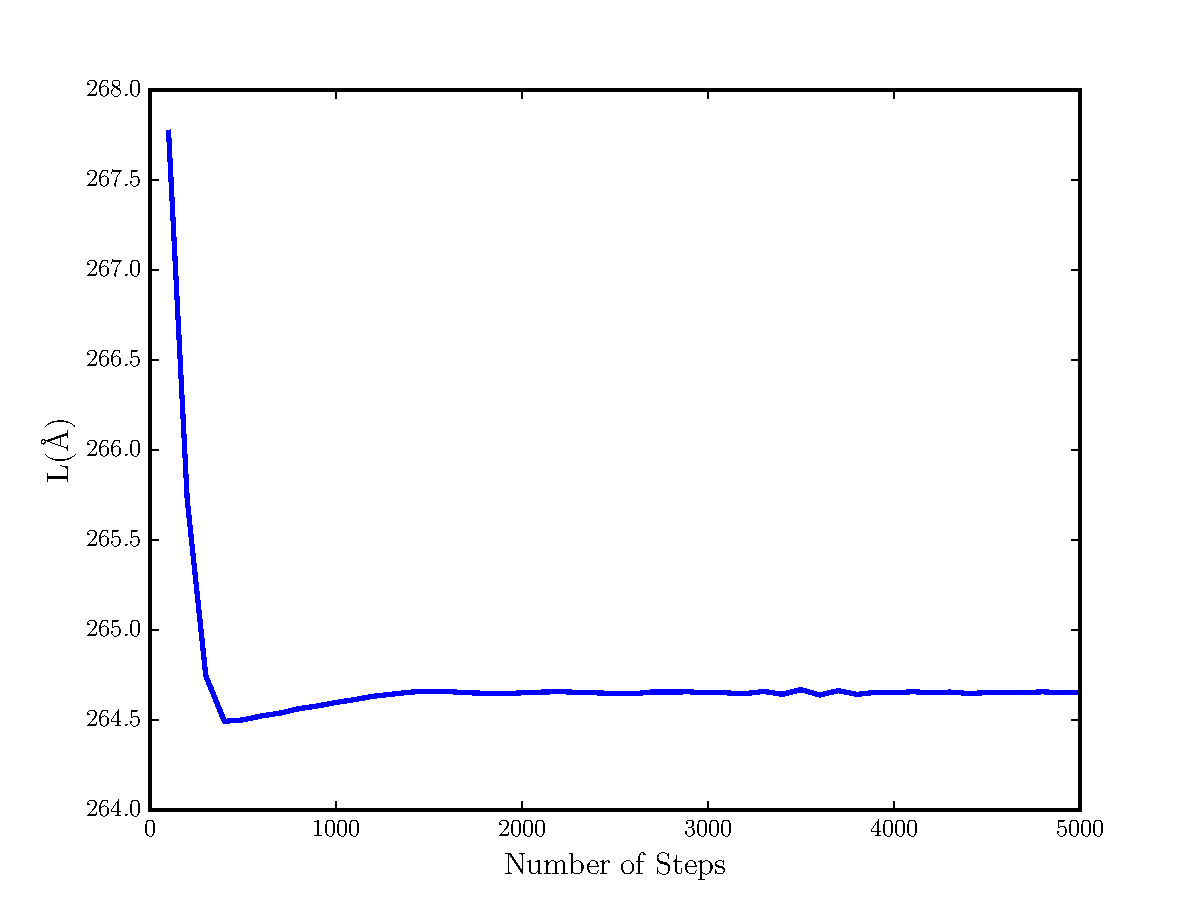
\includegraphics[width=0.45\textwidth]{./Figures/lx_npt}
  \\ (a) & (b)
  \end{tabular}
\caption{(a) A snapshot of the arrangement of atoms illustrating loss of
structural integrity of the Si bar. 
(b) Si bar length is plotted against the number of time steps during
the NPT ensemble stage of the simulation.}
\label{fig:dgsm1}
\end{center}
\end{figure}

\clearpage

%%%%%%%%%%%%%%%%%%%%%%%%%%%%%%%%%%%%%%%%%%%%%%%%%%%%%%%%%%%%%%%%%%%%%%%%%

\begin{figure}[p]
 \begin{center}
  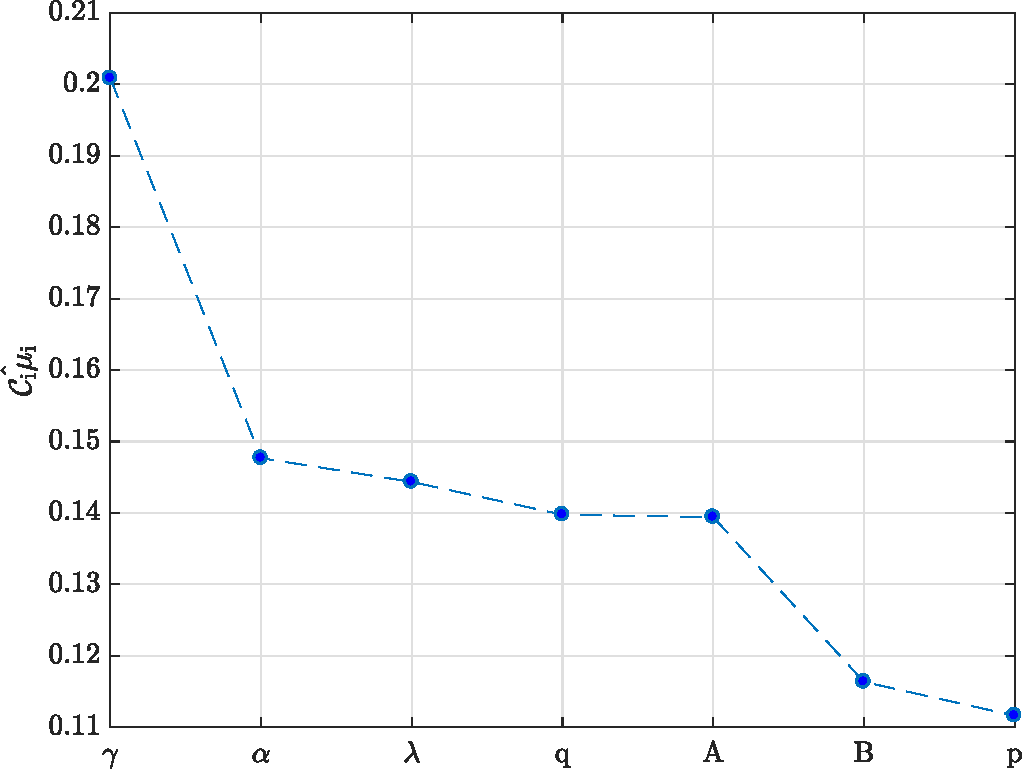
\includegraphics[width=0.70\textwidth]{./Figures/ub}
\caption{The quantity $\hat{\mathcal{C}_i\mu_i}$ as computed after 4 iterations and data at 25(7+1)
points is plotted for each SW potential parameter.}
\label{fig:screen}
\end{center}
\end{figure}

\clearpage


%%%%%%%%%%%%%%%%%%%%%%%%%%%%%%%%%%%%%%%%%%%%%%%%%%%%%%%%%%%%%%%%%%%%%%%%%




\end{document}
